\chapter{Optical Flow and Motion Estimation}
\label{ch:lesson21}

Optical flow estimates apparent motion between two frames of a video: for each pixel (or a chosen set of points), a 2D vector $(u,v)$ describing where it moved to. This chapter derives the classic \textbf{Lucas-Kanade} method from the same structure tensor used for corner detection in Chapter~\ref{ch:lesson20}, confronts the fundamental \textbf{aperture problem}, contrasts it with the globally-optimized \textbf{Horn-Schunck} method, and finishes with dense flow via the \textbf{Farneb\"ack} method.

\section{The brightness constancy assumption}

Optical flow assumes a point's intensity doesn't change as it moves: $I(x,y,t)=I(x+u,y+v,t+1)$. A first-order Taylor expansion of the right side gives the \textbf{optical flow constraint equation}:
\begin{equation}
I_x u + I_y v + I_t = 0,
\end{equation}
where $I_x,I_y$ are the spatial gradients (Chapter~\ref{ch:lesson12}) and $I_t$ is the frame-to-frame intensity difference. This is \textbf{one equation with two unknowns} ($u$ and $v$) at every single pixel --- not enough information on its own to solve for the flow.

\section{The aperture problem}

Looking through a small window at a moving edge, only the motion \textbf{perpendicular to the edge} is visible; motion \textbf{along the edge} produces no visible change at all, as Figure~\ref{fig:l21-1} demonstrates. This is exactly why the flow constraint equation is underdetermined: it only ever constrains the component of $(u,v)$ along the gradient direction $(I_x,I_y)$, leaving the perpendicular component completely unconstrained.

\begin{figure}[h]
\centering
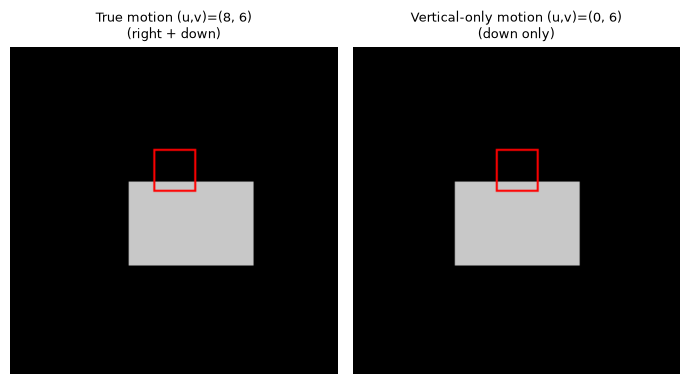
\includegraphics[width=0.7\textwidth]{figures/lesson21_fig01.png}
\caption{Two different true motions (right$+$down vs.\ down-only). Inside a small window straddling the rectangle's top (horizontal) edge, the two motions look pixel-for-pixel identical --- verified directly: a local measurement genuinely cannot tell them apart.}
\label{fig:l21-1}
\end{figure}

\section{Lucas-Kanade: solving the aperture problem with a window}

Lucas and Kanade's fix (\citelink{lucaskanade1981}{1981}): assume the flow $(u,v)$ is \textbf{constant over a small window}, then combine the flow constraint equation from every pixel in that window into an overdetermined least-squares system:
\begin{equation}
\underbrace{\begin{bmatrix}\sum I_x^2 & \sum I_xI_y \\ \sum I_xI_y & \sum I_y^2\end{bmatrix}}_{M}\begin{bmatrix}u\\v\end{bmatrix} = -\begin{bmatrix}\sum I_xI_t\\ \sum I_yI_t\end{bmatrix}.
\end{equation}
$M$ is exactly the structure tensor from Chapter~\ref{ch:lesson20}! This is not a coincidence: solving this system requires $M$ to be invertible, i.e.\ to have two large eigenvalues --- precisely the Shi-Tomasi ``good feature to track'' condition. A flat region ($M$ near zero) or an edge (one small eigenvalue --- the aperture problem again) gives an ill-conditioned or singular system; a corner gives a well-conditioned one. \textbf{Corners are trackable for exactly the same reason they're good corners.}

For a sub-pixel motion of $(0.6, 0.4)$ on a synthetic textured scene, a from-scratch Lucas-Kanade solve at 30 detected corners averages to $(0.612, 0.393)$ --- close to the true motion (Figure~\ref{fig:l21-2}).

\begin{figure}[h]
\centering
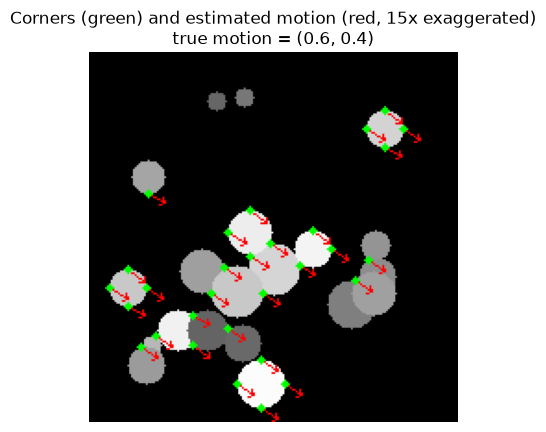
\includegraphics[width=0.5\textwidth]{figures/lesson21_fig02.png}
\caption{Corners (green) and estimated motion (red arrows, exaggerated $15\times$ since the true motion is sub-pixel).}
\label{fig:l21-2}
\end{figure}

\subsection*{Larger motions need iteration}

The single-shot linear solve relies on the Taylor approximation, which only holds for small motions. For a larger true shift of $(4.0, 3.0)$: the single-shot manual solve degrades badly, averaging to $(0.846, 0.690)$, while \code{cv2.calcOpticalFlowPyrLK} recovers it essentially exactly at $(4.000, 3.000)$, as shown in Figure~\ref{fig:l21-3}.

\begin{figure}[h]
\centering
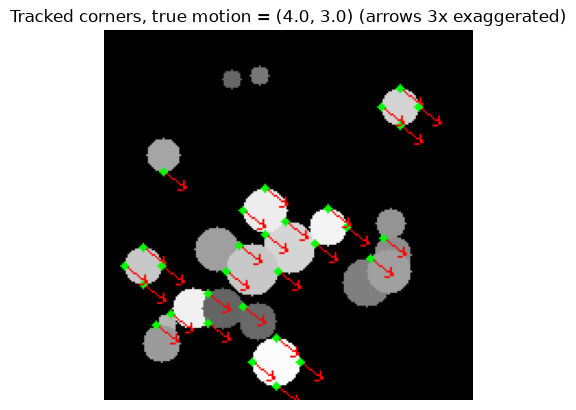
\includegraphics[width=0.9\textwidth]{figures/lesson21_fig03.png}
\caption{Tracked corners with a larger true motion, using \code{cv2.calcOpticalFlowPyrLK}.}
\label{fig:l21-3}
\end{figure}

OpenCV's \code{calcOpticalFlowPyrLK} handles large motions by running Lucas-Kanade \textbf{iteratively} (re-warping and re-linearizing until convergence) on an \textbf{image pyramid} (Chapter~\ref{ch:lesson11}) --- estimate coarsely on a small, blurry version of the image first, then refine level by level. This combination lets it recover large motions accurately even though the underlying linear approximation is only valid locally, one small step at a time.

\section{Horn-Schunck: a global alternative to windowed flow}

Lucas-Kanade's window is a \emph{local} smoothness assumption: flow is constant over a small neighborhood, estimated independently at each point. The same year, Horn and Schunck (\citelink{hornschunck1981}{1981}) proposed a \emph{global} alternative: instead of many independent per-window solves, minimize a single energy over the whole image at once, trading off how well the flow satisfies the optical flow constraint equation against how smoothly it varies between neighboring pixels:
\begin{equation}
E(u,v) = \sum_{x,y} \underbrace{(I_x u + I_y v + I_t)^2}_{\text{data term}} \;+\; \alpha^2 \underbrace{\left(\|\nabla u\|^2 + \|\nabla v\|^2\right)}_{\text{smoothness term}}.
\end{equation}
The smoothness term is what makes this global: it couples every pixel's flow to its neighbors', so minimizing $E$ (e.g.\ by iterative Gauss-Seidel updates) lets reliable flow estimates near edges \emph{propagate} into flat, textureless regions that have no local information of their own --- exactly the failure mode the aperture problem produces at its worst, as Figure~\ref{fig:l21-4} shows.

\begin{figure}[h]
\centering
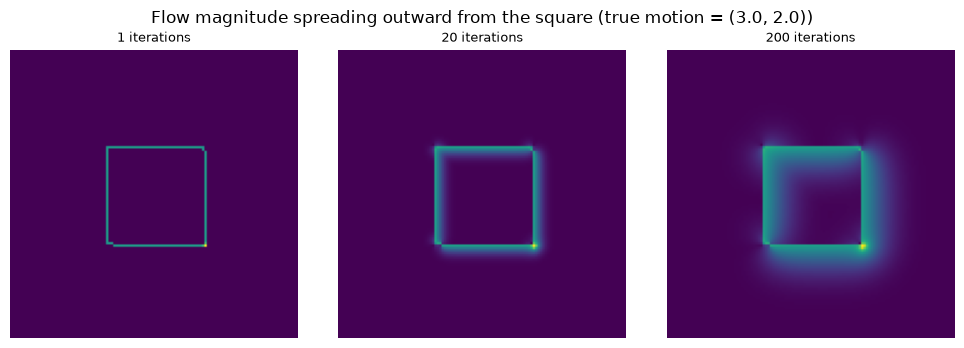
\includegraphics[width=0.9\textwidth]{figures/lesson21_fig04.png}
\caption{Flow magnitude spreading outward from a single textured square, after 1, 20, and 200 Gauss-Seidel iterations. After just 1 iteration, flow is only nonzero right at the square's edges; by 200 iterations it has spread well beyond, though still far from every pixel --- a real solver would run more iterations (or use a pyramid) to converge everywhere.}
\label{fig:l21-4}
\end{figure}

\section{Farneb\"ack's method for dense optical flow}

Horn-Schunck's global optimization is elegant but expensive and slow to converge; for dense (every-pixel) flow, Farneb\"ack's method (\citelink{farneback2003}{2003}) --- exposed as \code{cv2.calcOpticalFlowFarneback} --- is a more popular method actually used in practice. It stays local, like Lucas-Kanade, but drops the constant-flow-in-a-window assumption in favor of locally approximating each neighborhood with a polynomial and comparing the polynomial expansions between frames.

On a synthetic scene with true motion $(5.0,-3.0)$: averaging the dense flow over \emph{all} pixels gives a biased $(2.25,-1.35)$, but restricting to textured (high-gradient) pixels recovers $(5.00,-3.00)$ almost exactly. This is the aperture problem again, at its most extreme: over flat, textureless background, there's no local information at all to estimate motion from, dragging the whole-image average away from the true value. Figure~\ref{fig:l21-5} shows the resulting flow field.

\begin{figure}[h]
\centering
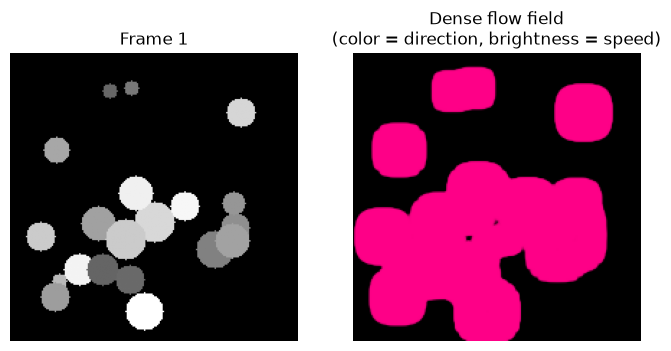
\includegraphics[width=0.85\textwidth]{figures/lesson21_fig05.png}
\caption{A synthetic frame and its dense Farneb\"ack flow field, visualized with color = direction, brightness = speed. Every moving circle produces the same color here, since they all share the same true motion.}
\label{fig:l21-5}
\end{figure}

\subsection*{A real video: the Army sequence}

On a real video with independently moving objects, this color-coding immediately separates different motions at a glance (Figure~\ref{fig:l21-6}) --- exactly why it's the standard way to visualize dense flow fields.

\begin{figure}[h]
\centering
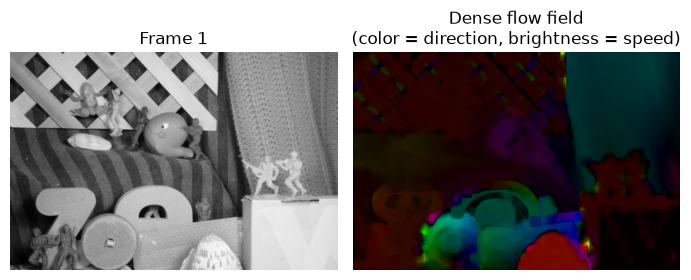
\includegraphics[width=0.85\textwidth]{figures/lesson21_fig06.png}
\caption{A frame from the Army sequence and its dense flow field. \attrib{Image source: \href{https://vision.middlebury.edu/flow/data}{Middlebury Optical Flow}.}}
\label{fig:l21-6}
\end{figure}

\subsection*{Exercises}
\begin{enumerate}
  \item Rerun the sparse Lucas-Kanade comparison with a true motion of $(10.0, 8.0)$. Does \code{cv2.calcOpticalFlowPyrLK} still recover it accurately? At what point (try increasingly large motions) does it start to fail, and why would you expect a pyramid to help push that limit further out?
  \item Modify the synthetic scene so the circles move with \emph{different} velocities (e.g.\ half moving one way, half another). Re-run the dense Farneb\"ack color visualization and confirm the two motions appear as two distinct colors.
  \item In the aperture-problem demo, construct a small textured (non-edge) patch instead of a straight edge, and show that \emph{both} components of an arbitrary motion vector are recoverable from it --- unlike the edge case, this should not have an invisible direction of motion.
\end{enumerate}

\vfill
\fullcode{lesson21}{lesson21_optical_flow}
